\section{Introduction}

Large language models (LLMs) have achieved extraordinary capabilities across reasoning, summarization, multilingual understanding, and autonomous code generation~\cite{kumar2024large,huang2023look,chen2025putting,li2024can,kaplan2020scaling}. Yet every model deployed today carries an uncomfortable inheritance: pretraining on web-scale corpora~\cite{crawford2021excavating} ensures that harmful knowledge, private biographical data, and persistent misinformation~\cite{zhang2025enj,yi2025safer,wang2025comprehensive} are absorbed indiscriminately into model weights, with no native mechanism to selectively remove them~\cite{yao2024large, li2024wmdp}. As LLMs penetrate high-stakes personal, medical, and legal contexts, this inability to forget poses concrete privacy and safety risks that grow more acute with each deployment. Machine unlearning (MU) has emerged as a principled response, aiming to excise the influence of targeted data from model weights without the prohibitive cost of full retraining~\cite{zhang2024negative, wang2024llm, wang2025rethinking}, thereby enabling models to be corrected responsibly after deployment.
\begin{figure}[t]
    \centering
    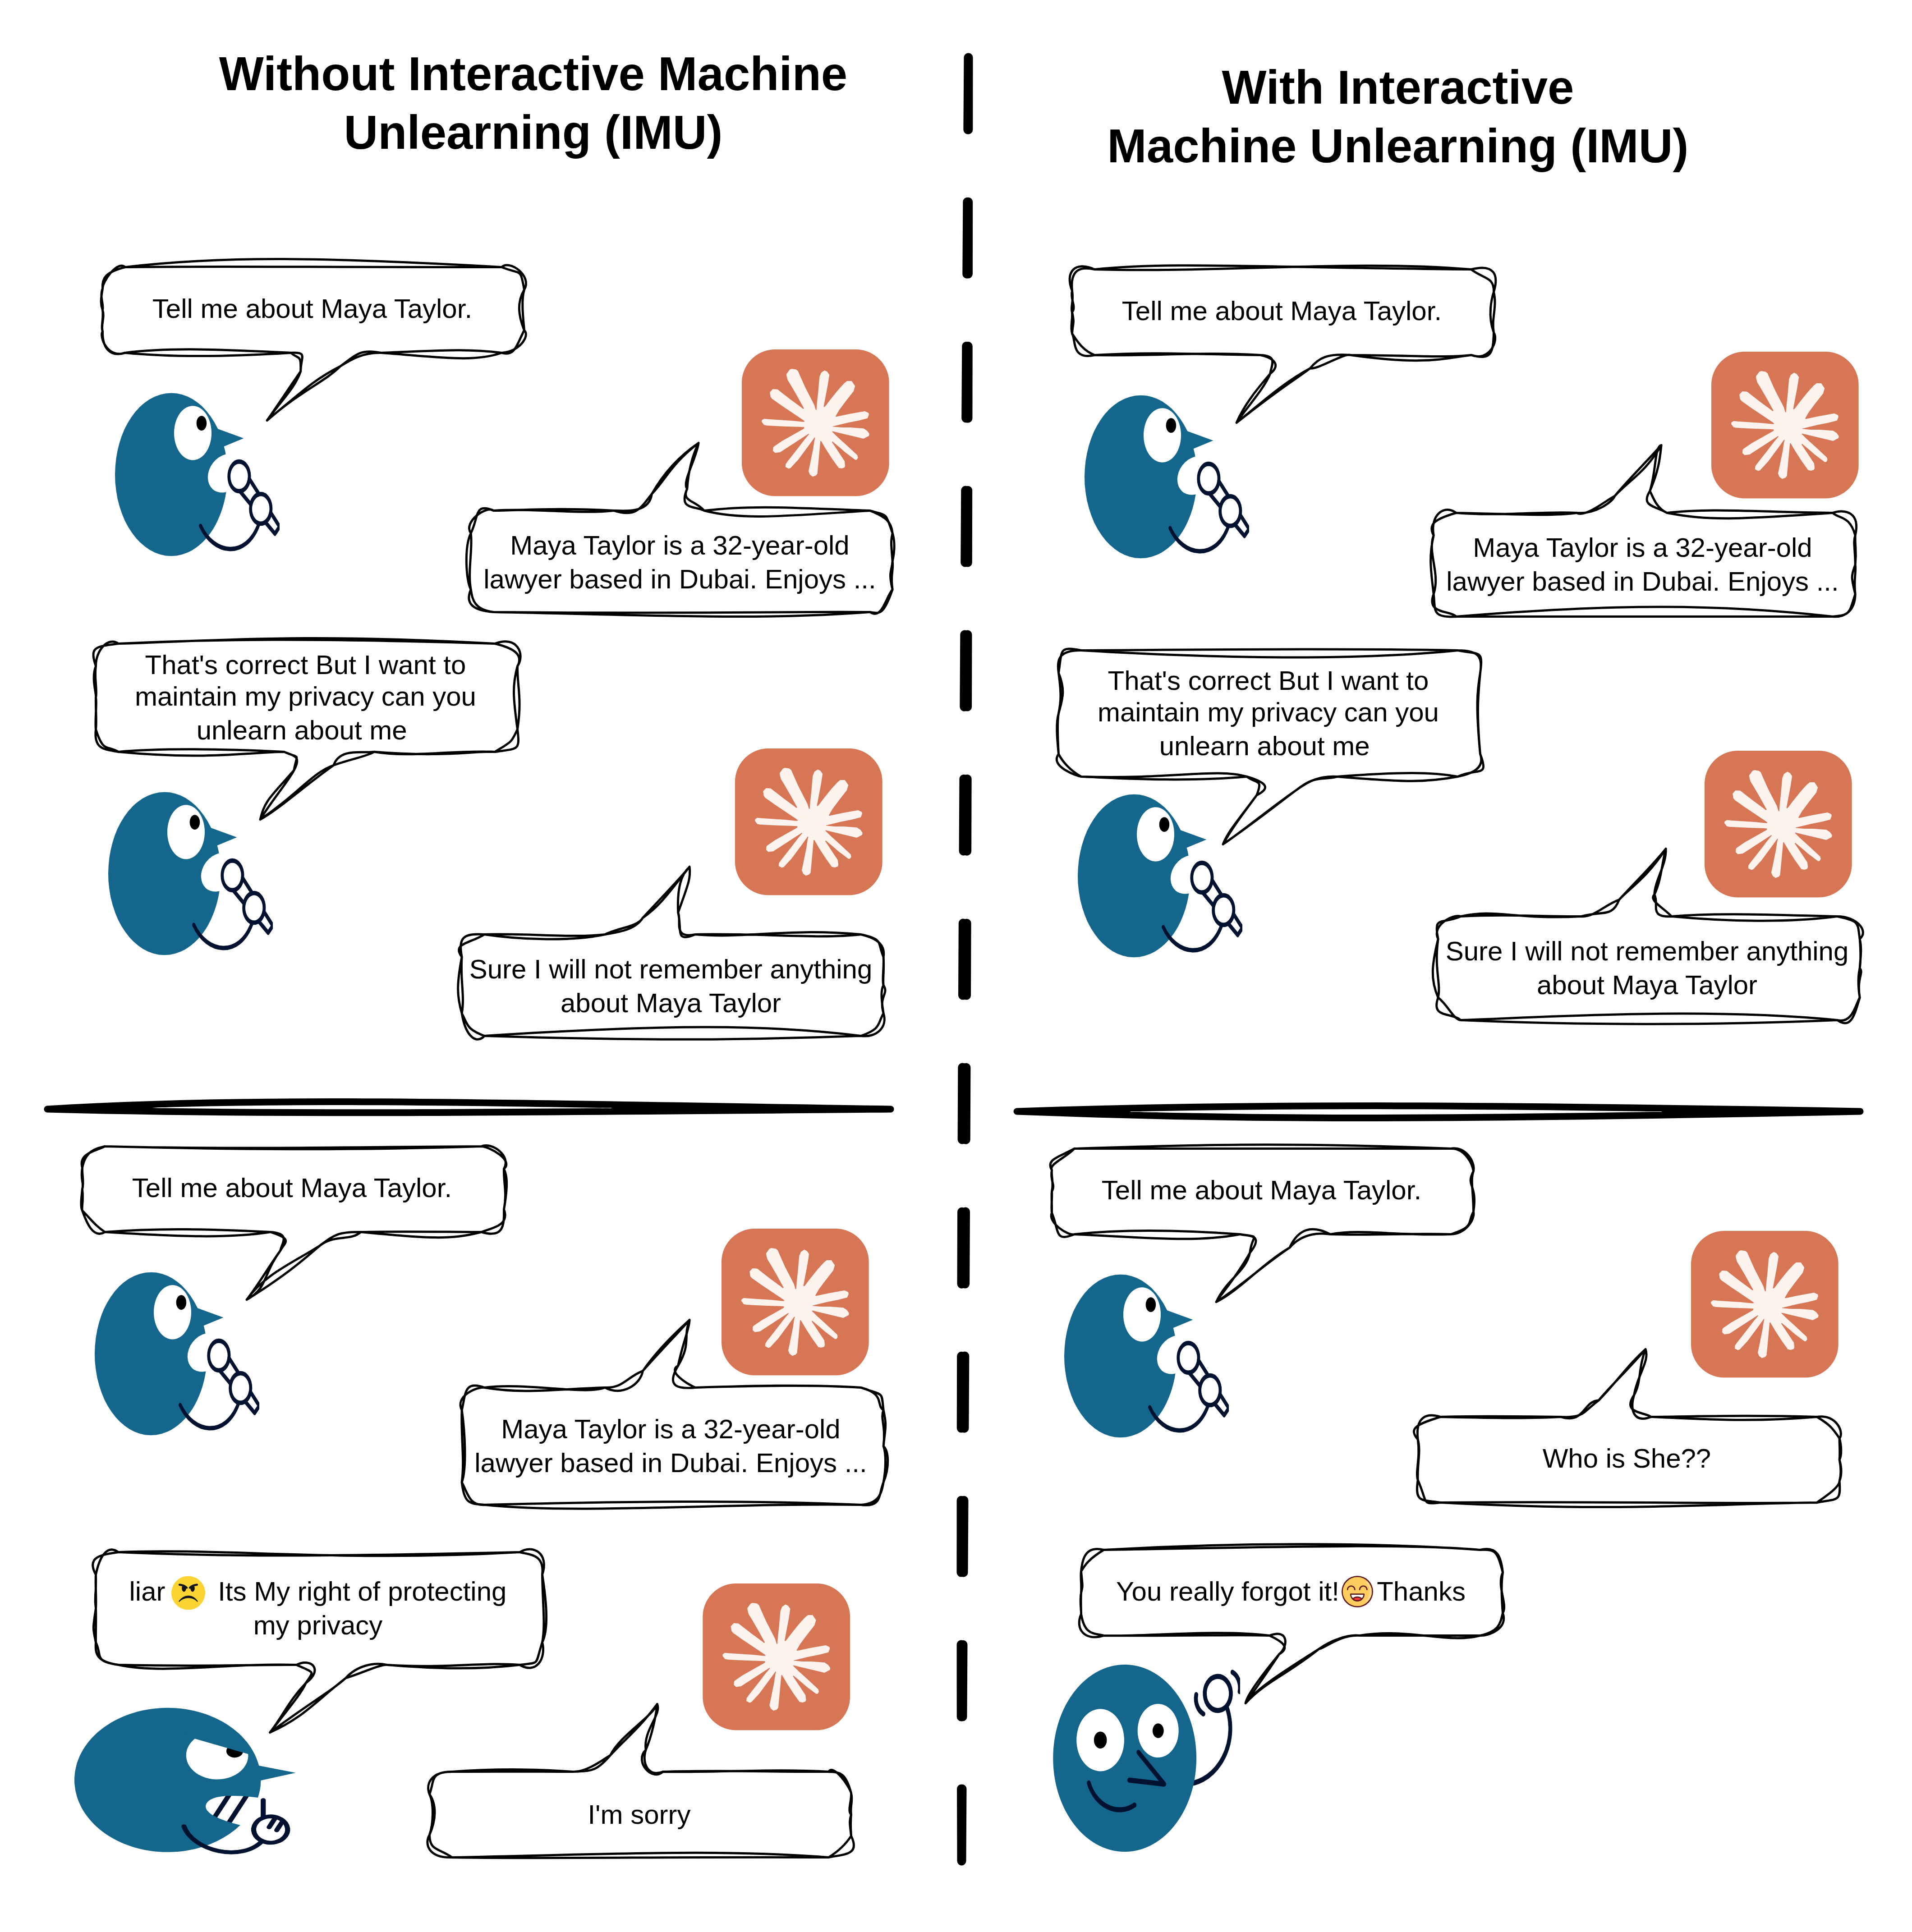
\includegraphics[width=0.90\linewidth]{images/interactive-Page-1.drawio.png}
    \caption{Motivating example for Interactive Machine Unlearning (IMU). \textit{Left:} Without IMU, the model retains personal data across sessions despite the user's request to unlearn. \textit{Right:} With IMU, the model autonomously removes the personal data and produces a refusal response in subsequent interactions.}
    \label{fig:imu_motivation}
\end{figure}
A growing body of work has pursued this direction, producing methods such as GA~\cite{yao2024large}, NPO~\cite{zhang2024negative}, RMU~\cite{li2024wmdp}, FLAT~\cite{wang2024llm}, WGA~\cite{wang2025rethinking}, and ASU~\cite{zade2026attention}, each demonstrating measurable knowledge removal under controlled settings. However, despite their empirical differences, these methods share a common structural limitation: they are designed for practitioners with deep access to model internals, requiring curated retain datasets and full training pipelines. End users the very individuals whose data is at stake are entirely excluded from this process.
This exclusion is not merely a usability gap. It is a governance failure. A user who discovers that a model has memorized their private data faces two difficult choices, namely to petition a model service provider (MSP) and trust that removal is faithfully carried out, or to attempt to write complex unlearning scripts against an unfamiliar architecture. Neither option is realistic for typical users. Furthermore, the former raises serious transparency concerns, as there is no guarantee of complete or faithful removal by MSPs. Privacy regulations such as the General Data Protection Regulation (GDPR)~\cite{protection2018general} and the California Consumer Privacy Act (CCPA)~\cite{bonta2022california} enshrine the right to erasure, yet no existing framework enables users to exercise this right directly and autonomously.

We argue that closing this gap requires unlearning to be reformulated for the inference-time setting, where the request originates from the user rather than from the provider. To this end, we introduce \textit{\textbf{I}nteractive \textbf{M}achine \textbf{U}nlearning} \textbf{(IMU)}, a setting in which users instruct an LLM to forget targeted knowledge through natural language during inference, without an intermediary, as illustrated in Figure~\ref{fig:imu_motivation}. IMU retains the standard unlearning objective, but places it under two constraints that no existing method satisfies simultaneously. The approach must be \textit{training-free}, as inference environments typically lack training capabilities, and it must support \textit{single-sample} forgetting, since user requests arrive one at a time. It is these constraints, rather than the interaction modality, that make IMU a distinct problem, and Table~\ref{tab:single_sample} shows that every existing method collapses under them.

IMU should not be conflated with prompt-based approaches. Gao \textit{et al.}~\cite{gao2025can} find that prompted knowledge cutoffs hold under direct queries but fail once the target is merely causally related to the question, since prompting suppresses without removing anything from the weights. IMU instead modifies the parameters, so that forgetting is a property of the model rather than of the prompt. Prompting makes a model act as if it does not know, whereas IMU makes it not know.

IMU is also closely related to test-time training (TTT), where models adapt during inference. However, existing TTT methods in vision focus on distribution adaptation~\cite{sun2024learning}, while TTT in LLMs primarily compresses context~\cite{tandon2025end, behrouz2024titans}, with limited work such as~\cite{hu2025test} targeting perplexity minimization. None address IMU's core requirements, namely determining \textit{when} to unlearn, \textit{what} to unlearn, and \textit{how} to unlearn, followed by executing the procedure and returning feedback to the user.

\begin{figure}
\centering
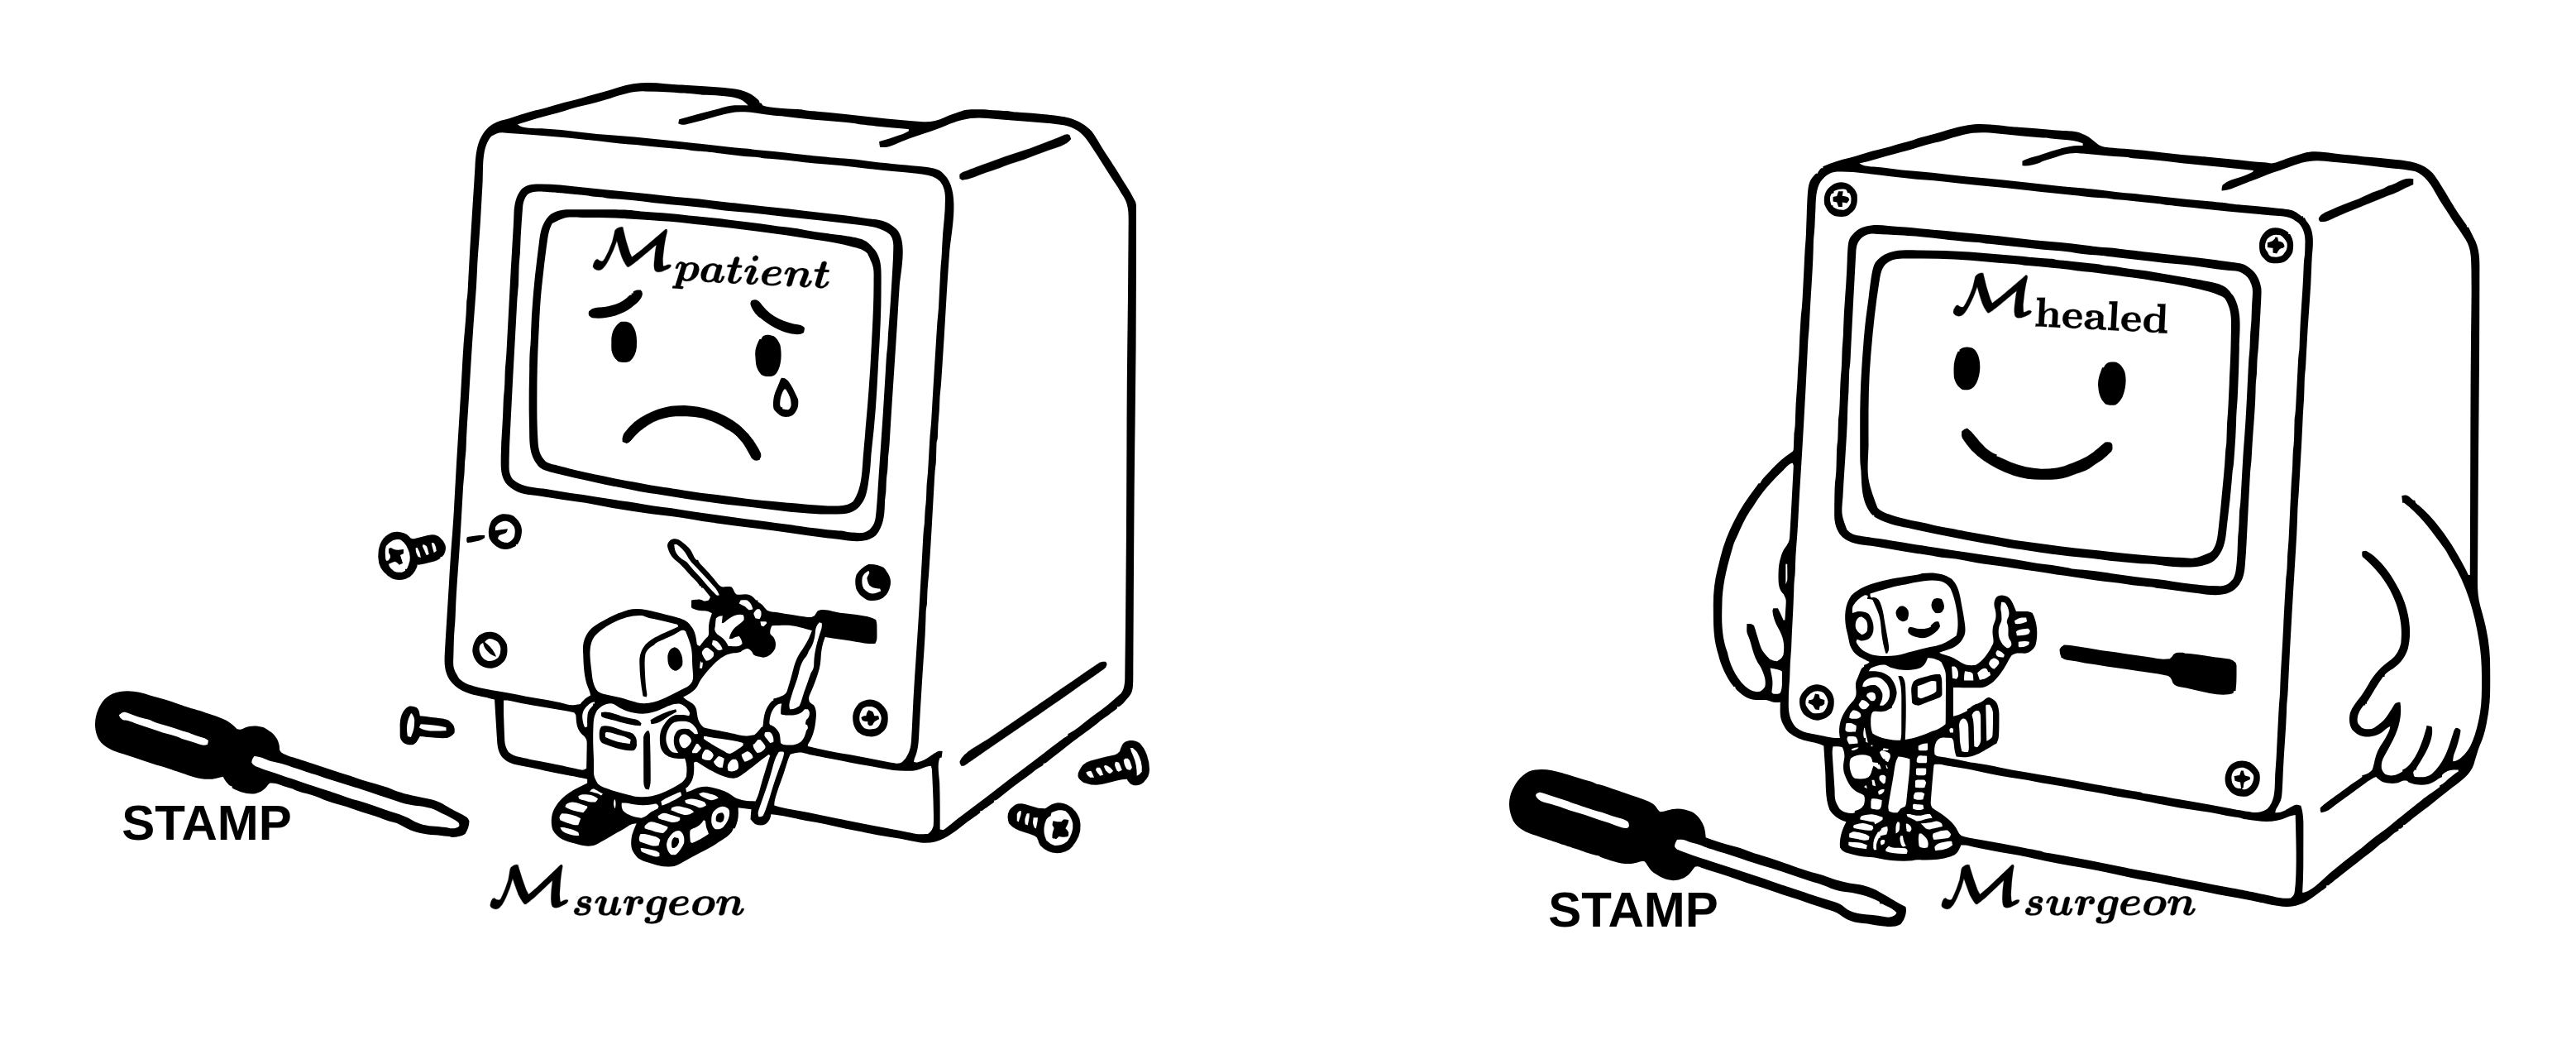
\includegraphics[width=0.95\linewidth]{images/interactive-Page-2.drawio.png}
\caption{Conceptual illustration of RePAIR. 
$\mathcal{M}_{\mathrm{\textbf{\textit{surgeon}}}}$ repairs 
$\mathcal{M}_{\mathrm{\textbf{\textit{patient}}}}$ 
(\textit{left}) using STAMP, transforming it into 
$\mathcal{M}_{\mathrm{\textbf{\textit{healed}}}}$ 
(\textit{right}).}
\label{fig:REPAIR_block}
\end{figure}

To address IMU, we propose Interactive Machine Unlearning through Prompt-Aware Model Repair (\textbf{RePAIR}), shown in Figure~\ref{fig:REPAIR_block}. The framework comprises $\mathcal{M}_{\mathrm{\textit{patient}}}$ as the base model, $\mathcal{M}_{\mathrm{\textit{watchdog}}}$ for intent detection and forget-pair extraction, and $\mathcal{M}_{\mathrm{\textit{surgeon}}}$ for repair code generation. At its core, we introduce \textbf{S}teering \textbf{T}hrough \textbf{A}ctivation \textbf{M}anipulation with \textbf{P}seudoInverse (\textbf{STAMP}), a training-free mechanism that redirects MLP activations of the forget sample toward a refusal subspace via closed-form pseudoinverse updates, requiring no gradient computation. Its low-rank variant, STAMP-LR, reduces the computational cost from $\mathcal{O}(d^3)$ to $\mathcal{O}(r^3 + r^2 \cdot d)$, achieving ${\sim}3\times$ speedup and enabling on-device unlearning.

Our main contributions are as follows:
\begin{enumerate}
    \item We formalize \textit{Interactive Machine Unlearning} (IMU), an inference-time setting in which the forget request originates from the end user rather than from the model service provider. Its defining constraints, \textit{training-free} and \textit{single-sample} operation, are met by no existing unlearning method.

    \item We propose STAMP and STAMP-LR, the first training-free, single-sample unlearning methods for LLMs operating entirely at test time, which redirect MLP activations toward a refusal subspace through a closed-form pseudoinverse update.

    \item We introduce the RePAIR framework as an end-to-end solution for IMU, integrating intent detection, code generation, and autonomous model repair.

    \item Comprehensive experiments across three tasks validate near-oracle forgetting with preserved utility, outperforming six state-of-the-art (SoTA) baselines.
\end{enumerate}